\section{Integration with other tools}
\label{sec:integration}

\todo{do we want to merge this into the ``practice'' section?}

\subsection{Integration with the LKB Workbench}
\label{sec:integration-lkb}

\begin{figure}
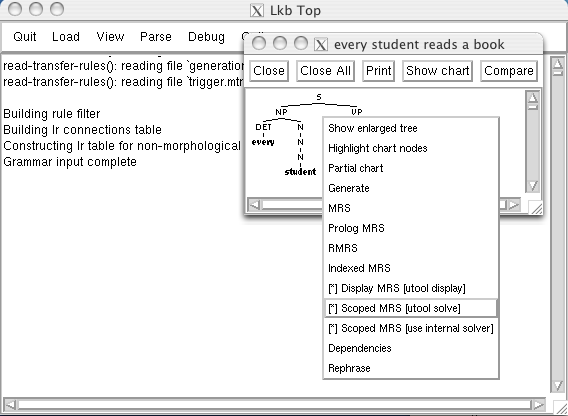
\includegraphics[width=\textwidth]{lkb-integration}
\caption{Calling Utool from an LKB context menu.
\label{fig:lkb-integration}}
\end{figure}

Utool can be used as a drop in replacement for the MRS constraint
solver built into the LKB system. The distribution contains a Lisp
file \verb|lkb-utool.lisp| that can be simply loaded into a running
LKB session and replaces the internal constraint solver.

Alternatively, the file \verb|lkb-utool-menu.lisp| can be loaded into
a running LKB session, which extends the context menu which shows up
when clicking on a parse tree with two commands:

In both cases, utool has to run in server mode listening in the
standard port 2802.

\subsection{Writing your own client for the Utool Server}

The following perl script illustrates how to implement a utool client.
The script assumes that an utool process runs in server mode on the
local machine listening on the standard port 2802.

\begin{verbatim}
use IO::Socket;

# read a dominance constraint
$message = join('', <>);

# open connection
$socket = IO::Socket::INET->new("localhost:2802") or die $!;

# and send it to the server
print $socket <<EOF;
<utool cmd='solve' output-codec='term-oz'>
  <usr codec='domcon-oz' string='$message'/>
</utool>
EOF

# shutdown connection
$socket->shutdown(1);

# print the answer 
while (<$socket>) { print }
\end{verbatim}

The script reads a dominance constraint from standard input, opens a
connection to the server and sends the dominance constraint to the
server. The answer -- in this case a list of solved forms -- is then
printed to the standard output.

A slightly extended version of the above script can be found
\todo{wo?}.


%%% Local Variables: 
%%% mode: latex
%%% TeX-master: "0"
%%% TeX-command-default: "LaTeX"
%%% End: 
